\documentclass[12pt]{article}

% 导入中文支持的包
\usepackage[UTF8]{ctex} % ctex 包支持中文处理

% 设置页面布局(可选)
\usepackage[a4paper,margin=1in]{geometry}

% 导入常用包(根据需要添加)
\usepackage{amsmath, amssymb} % 数学公式
\usepackage{booktabs} % 提供高级表格线
\usepackage{multirow} % 单元格合并
\usepackage{array} % 表格排版控制
\usepackage{graphicx} % 插入图片
\usepackage{hyperref} % 超链接
\hypersetup{
    colorlinks=true, % 激活链接颜色
    linkcolor=blue, % 文档内部链接颜色,适用于图、表在文中的引用
    citecolor=blue, % 文献引用链接颜色,适用于文中参考文献引用
    urlcolor=blue  % 外部URL链接颜色,适用于参考文献添加超链接
}
\usepackage{xcolor} % 颜色支持

% 标题和作者信息(可选)
\title{颅内压生理学和脑脊液动力学的仿体模型}
\author{王成}
\date{\today}

\begin{document}

% 标题
% \maketitle
% \newpage

% 目录(可选)
% \tableofcontents
% \newpage
\begin{center}
    \Large\textbf{生理性颅内压和脑脊液动力学的仿体模型}
\end{center}

% 正文
\begin{center}
    \section*{摘要}
\end{center}

我们在此描述了一种新颖的与颅腔等大的仿体模型,并给出了其验证过程。包括脑室、池区和蛛网膜下腔在内的脑脊液区域由核磁共振成像获得。
脑的机械特性和颅脊顺应性是基于已发表的数据设定的。实现了对脑脊液流动进行整体和脉动的生理建模。通过将模型中的流量和压力测量结果与健康受试者的体内数据进行比较来验证模型有效性。
脑室内记录的生理颅内压平均为10 mmHg,脉冲峰值幅度为0.4 mmHg。在大脑导水管和蛛网膜下腔中分别测得脑脊液流速峰值为0.2和2 ml/s。
本模型是一种首次尝试在体外模拟生理颅内动力学的方法。在此,我们描述了模型的设计和制造,操作参数的定义和实现,以及所模拟动力学的验证。

索引术语——解剖模型,顺应性,蛛网膜下腔(SAS),脑室系统。

\section*{\uppercase\expandafter{\romannumeral1}.引言}

脑脊液(CSF)有助于中枢神经系统(CNS)的体内平衡。在颅腔中,由于受到大气压强的作用,脑脊液被局限在脑室和蛛网膜下腔(SASs)中。
脑脊液通过浮力支撑大脑,保护其免受冲击,输送营养物质和神经内分泌物质,并清除代谢废物。

CSF动力学的变化与多种疾病有关。例如,脑积水和脊髓空洞症已被证明与CSF总体流动及脉动的紊乱有关。然而,这些关系的具体细节尚不清楚。

颅内动力学模型可以提高对中枢神经系统病理生理学的理解。集总参数和计算流体动力学(CFD)模型均已用于表征CSF空间以及主要颅内动脉的动力学特征。
集总参数方法特别适合用于颅内动力学的整体经验描述。相应的模型参数,如脑脊液流出阻力和压力-体积指数,在过去的十年中已成为临床实践中的标准。
另一方面,CFD模型可以用于获取通过测量无法获得的空间分辨流动信息。

然而,无论是集总参数模型还是CFD模型都未被证明是开发及优化颅腔动力学相关医疗器械的理想选择。
例如,用于治疗脑积水的脑脊液分流器根据ISO 7197标准通过实验方式进行测试以评估液压阻力。
然而,除了伦理问题,比起小鼠、老鼠或兔子,尤其是当使用诸如狗、山羊或猴子等脑内动力学与人类更为接近的大型动物时,实验成本将会非常昂贵。
体外模型代表了第四种可能有助于研究中枢神经系统病理生理学的模型类型。解剖细致和简化的模型都已被用于验证MRI序列、脑力学的计算模型,以及第三脑室中脑脊液流动。在脑损伤研究中,模型被用于研究组织对冲击的反应。
据我们所知,仅有一个关于脊柱脑脊液空间中流体和压力动态的模型被报道过;该模型被用于理解脊髓空洞症。

颅内空间的仿体模型有可能减少、改进,并在较小程度上取代动物模型用于分流器和其他神经外科器械的测试。
实现此类应用的一个重要步骤是复制健康状态下的颅内动力学。我们在此展示了首创的颅内腔体仿体模型,该模型能够再现生理性的脑脊液和压力动态。
我们报告了模型的设计、开发及与文献中描述的体内数据的验证,显示这种建模方法可以促进对颅内动力学的理解。

\section*{\uppercase\expandafter{\romannumeral2}.材料与方法}

\subsection*{A. 脑脊液和脑室系统}
我们使用以下方法在硅胶大脑中构造了一个脑室系统:对 27 岁健康男性志愿者采集的 MRI 数据进行3D重建,为设计模型的脑室区域提供了解剖学参考。
将脑室系统简化以获得适合铸造的矢状对称性:利用计算机辅助设计(CAD)软件(NX 7.5,西门子PLM软件,美国德克萨斯州普莱诺)将侧脑室合并为单一脑室表示;Monro孔被统一为通向第三脑室的单一连接器;Luschka孔和Magendie孔也被合并为单一通道。
这个简化的脑室区域的负模通过3D打印在Eden350V光聚合物打印机(Objet Geometries公司,美国马萨诸塞州比勒里卡市)上制造为两个矢状对称的半部分。

在获得脑室空间的正像(见第II-B节)后,将一个内径为2毫米的硅胶管插入到大脑导水管中,以避免其在模拟体构建期间发生形变。
为了模拟脑室中的脑脊液生成,在脑室系统的顶部建立了一个接入端口。这个接入端口也用于脑脊液空间的初步填充。在大脑导水管的顶部和底部建立了两个压力感应接入点。
改进的脑室系统如图\ref{fig:ventricular_system}所示,简化的效果在第IV节讨论。
\begin{figure}[h]
    \centering
    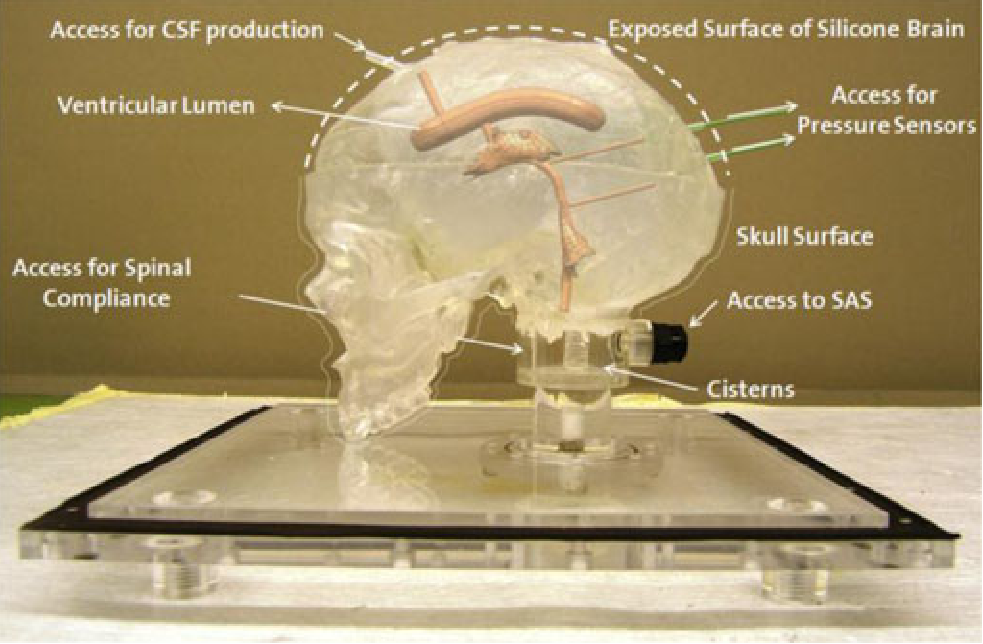
\includegraphics[width=0.7\textwidth]{Figures/1.png}
    \caption{模型的颅域。硅质大脑被容纳在塑料人类颅骨内。简化脑室系统的腔内显示为CAD模型的叠加。}
    \label{fig:ventricular_system}
\end{figure}
\subsection*{B.大脑和颅骨}
使用Sylgard 527,A&B绝缘硅胶(陶氏康宁,密歇根州米德兰)制成了一颗真人大小的硅胶大脑。先前的研究表明,这种材料在静态变形和动态加载高达10Hz时具有类似大脑的机械行为。
硅胶是围绕两个脑室负半部分铸造的。
固化后,负片被移除,左右脑部件用相同的硅胶粘在一起。在脑室壁上涂上一层标准铸造硅胶,以防止在坍塌时粘连。

完整的大脑被放置在一个已经移除上部的塑料人类头骨模型内(3B Scientific,德国汉堡)(见图\ref{fig:ventricular_system})。
\begin{figure}[h]
    \centering
    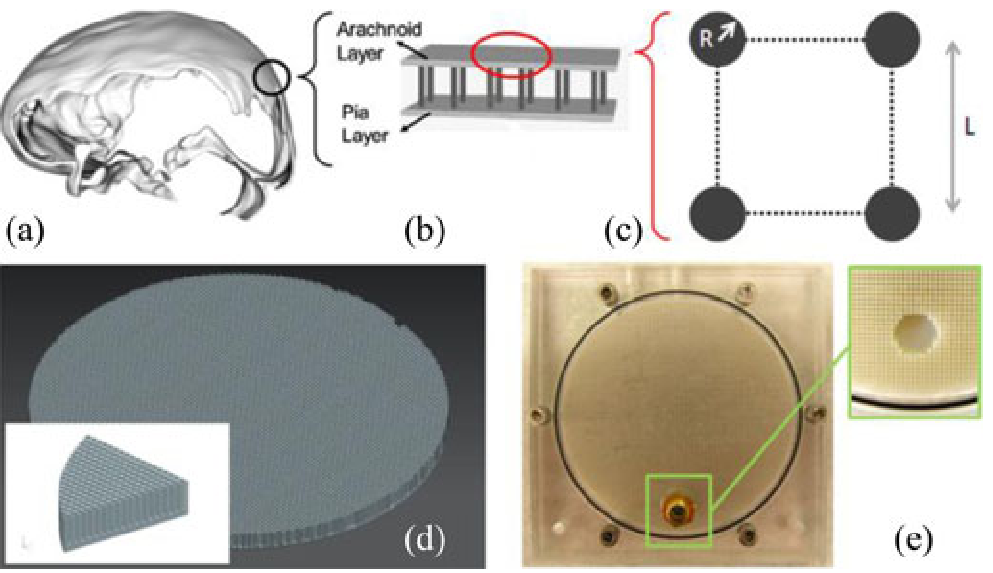
\includegraphics[width=0.6\textwidth]{Figures/2.png}
    \caption{SAS隔室设计。采用统一的模块化柱状结构以实现体内液力阻力值。 (a) SAS 宏解剖学。 (b) 理想化的柱状结构代表 SAS 微解剖学。 (c) 代表性单元格的顶视图。 (d) SAS 隔室的 CAD 设计。 (e) 3-D 打印的 SAS 表示和连接到模型的脑脊液池 (参见图 4)。}
    \label{fig:silicone_brain}
\end{figure}

\begin{figure}[h]
    \centering
    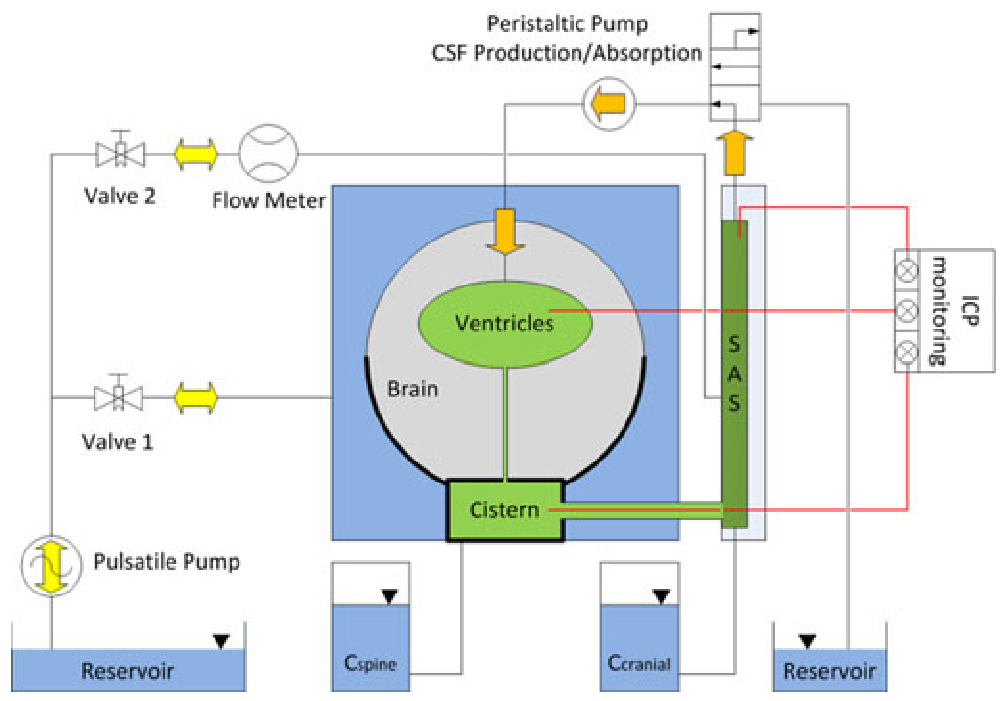
\includegraphics[width=0.7\textwidth]{Figures/3.png}
    \caption{仿真体设置示意图。脑室被包裹在硅胶大脑中,并连接到脑池和蛛网膜下腔。脑脊液产生和吸收速率可被控制。脑脊柱和颅脑顺应性单位分别连接到脑池和蛛网膜下腔。脉动流和颅内压在指示的位置监测。黑色三角形表示水-空气界面。}
    \label{fig:model_assembly}
\end{figure}
\subsubsection*{C.蓄水池与SAS}
脑脊液的整体流动起始于脑室,继续流向颅底的池,最终到达脊髓和皮质蛛网膜下腔(SAS),在那里大部分被重吸收至静脉血中。
SAS 的微观结构影响脑脊液动力学。微观结构的影响可以通过其水力阻力的空间平均和表示,而水力阻力与渗透率有关。
据报道,SAS 的渗透率范围在$10^{-9}$到$10^{-7}$平方米之间。我们使用了平行板之间的均质柱结构(见图\ref{fig:silicone_brain})来解释 SAS 的水力阻力。
在这样的结构中,渗透率$k$是柱半径$r$和空隙率$\varepsilon$的函数:
\begin{equation}
    \frac{k}{r^2} = \frac{\pi \varepsilon \left(1 - \sqrt{1 - \varepsilon}\right)^2}{24 \left(1 - \varepsilon\right)^{3/2}} \quad \text{and}
\end{equation}

\begin{equation}
    \varepsilon = \frac{V_{\text{fluid}}}{V_{\text{tot}}} = \frac{L^2 - \pi r^2}{L^2}
\end{equation}

$L$是相邻代表性单位单元之间中心距离,我们选择了$r = 0.5$毫米和$L = 1.5$毫米的配置,根据(1)和(2)得到了$1.7×10^{−8}$平方米的磁导率值。
这种柱状构型是通过3D打印(Eden350V,Objet Geometries Inc.)制造的,并放置在聚甲基丙烯酸甲酯(PMMA)外壳中,以123.7毫升的体积代表其颅内空腔系统,根据体内MRI数据(见图2)。
SAS区被连接到24毫升容积的圆柱腔,代表了基底池空间(见图1)。这种模块化方法允许简单地改变SAS阻力,以应对可能导致SAS阻塞的病理情况,如出血。

\begin{figure}[h]
    \centering
    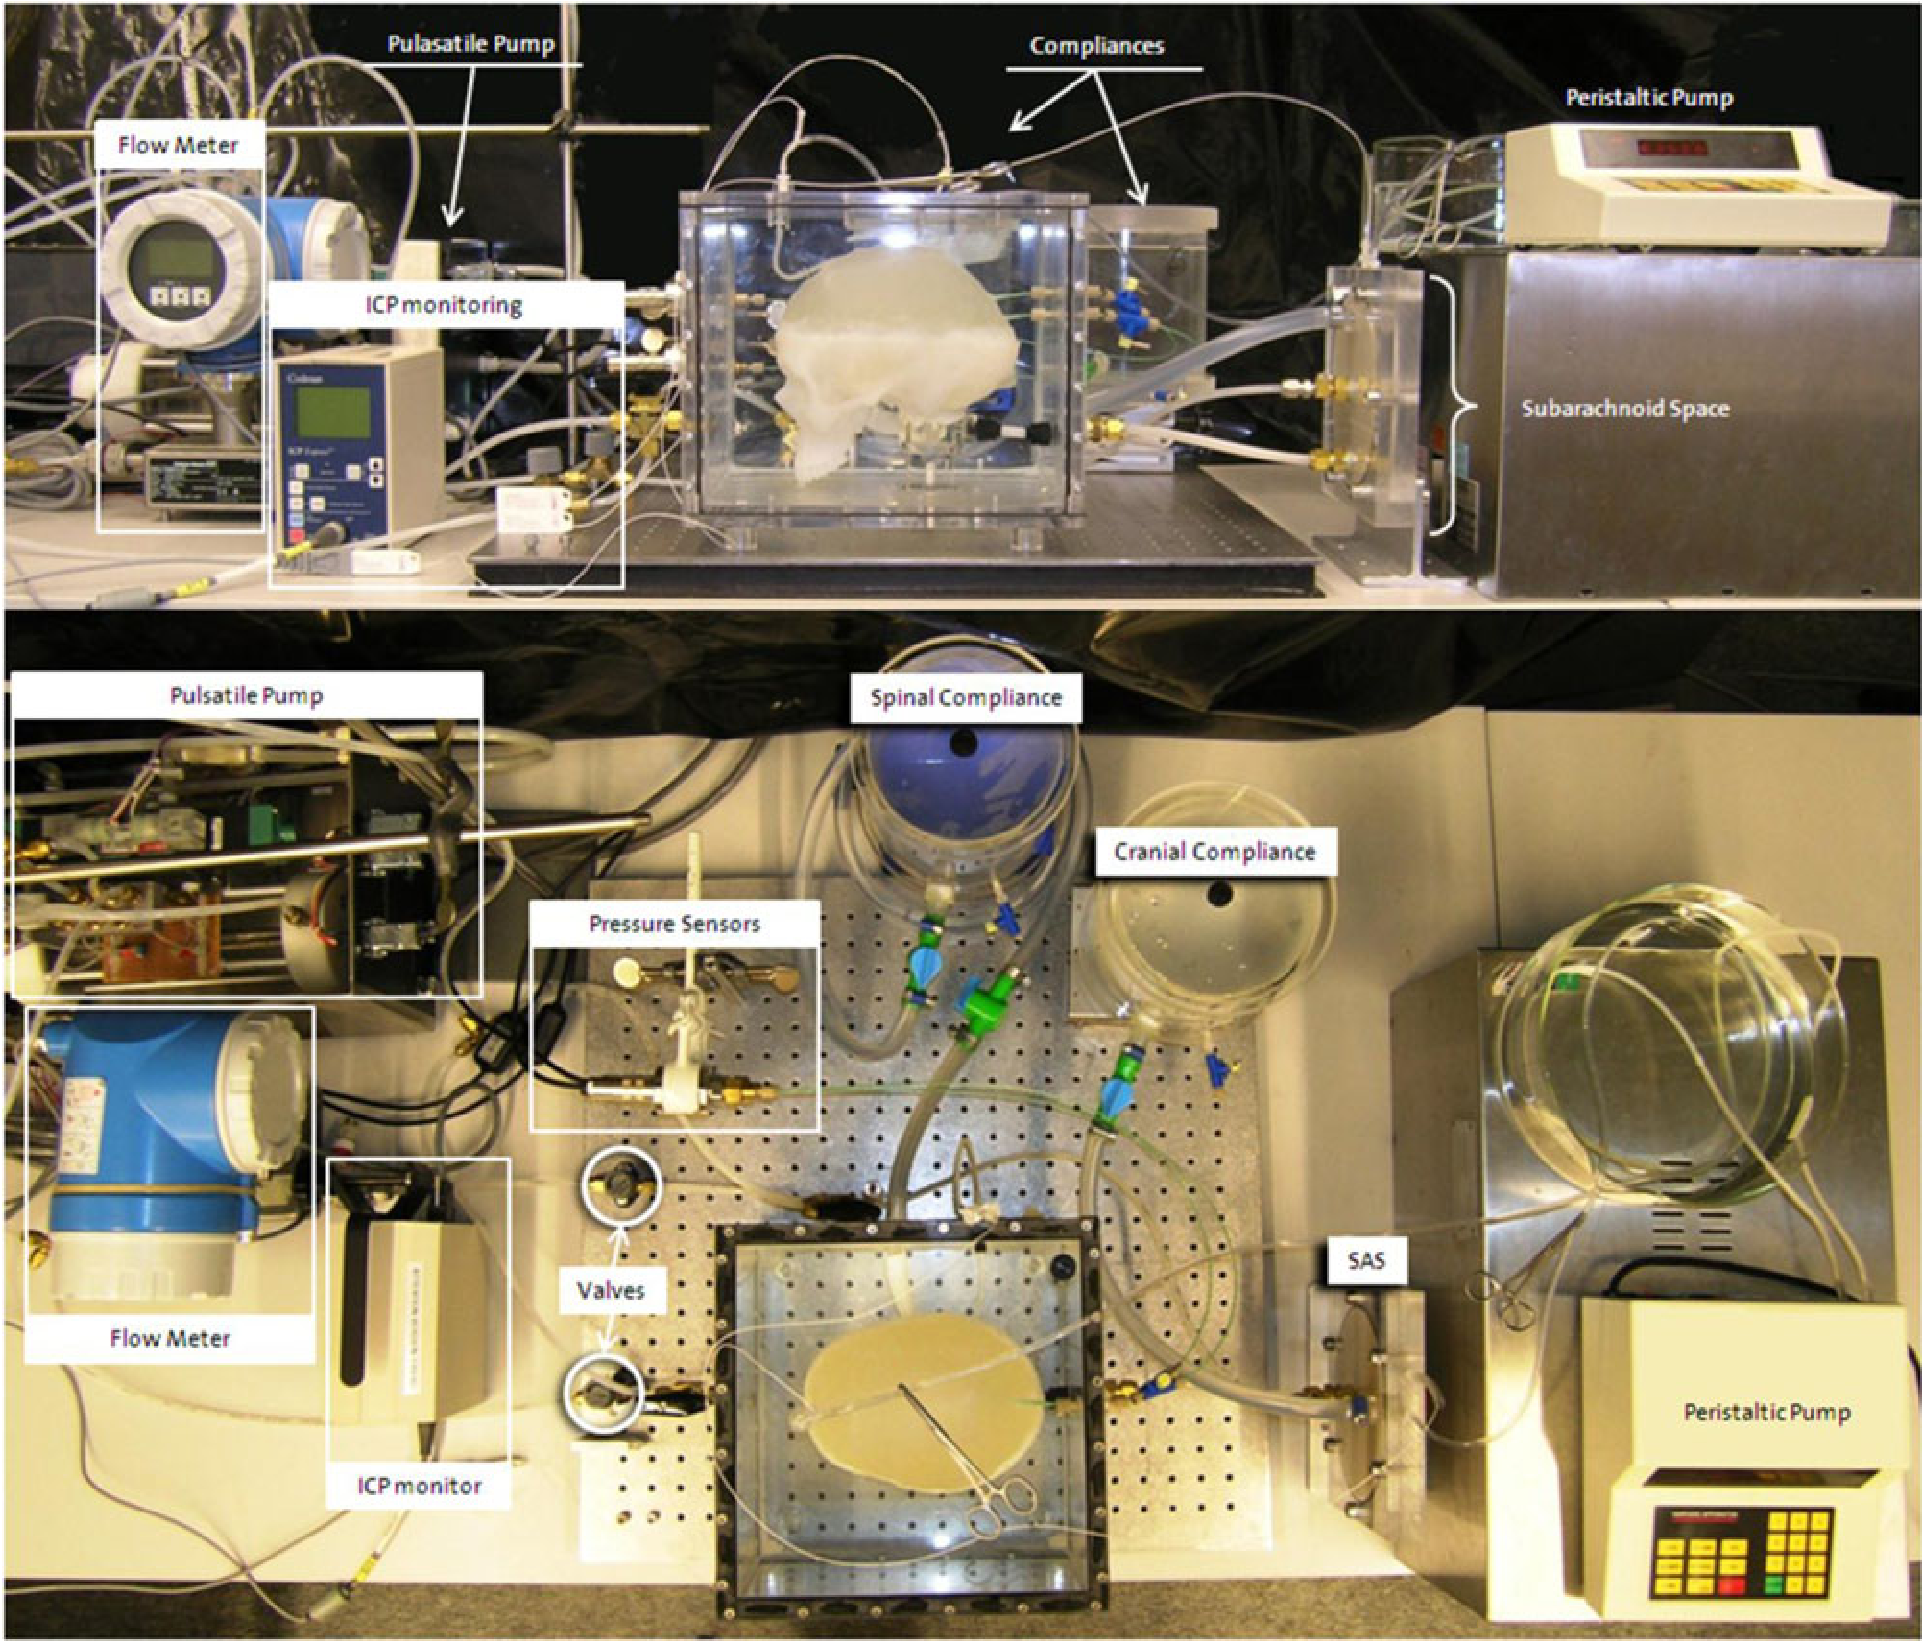
\includegraphics[width=0.9\textwidth]{Figures/4.png}
    \caption{模型设置。顶部:正面视图。 底部:俯视图。 模型的颅域放置在PMMA箱中,并被水所包围。 显示了激励和采集系统的组件,以及顺应性和SAS隔室。 模型设置的组件成本约为43,000美元。}
    \label{fig:csf_flow_path}
\end{figure}

除了SAS表征和合规模块(见第II-D节)外,所有颅内元素包括头骨、硅胶脑、池和脑室腔都封闭在一个注满水的PMMA盒子中(见图3和图4)。
水不仅可以模拟动物实验中观察到的脑部浮力效应,还可作为从脉搏泵(见II-E节)传递压力脉冲到颅内隔室的传输介质,模拟动脉脉动的效果。

\subsection*{D.顺应性}
颅脊系统的顺应性C被定义为其体积V随其压力P变化而变化的程度。
\begin{equation}
    C = \frac{dV}{dP}
\end{equation}
顺应性可以通过灌注实验来测量。顺应性可由此推导出的生理压力-体积关系大致如下:
\begin{equation}
    ICP = P_0e^{KV} + P_1
\end{equation}
$P_r = P_0 + P_1$代表输注前的静息颅内压(ICP)水平,$K$代表脑弹性系数。
据报道,健康人类的$K$可在 0.0886 到 0.177 $\mathrm{ml}^{-1}$之间变化,
对应于未受干扰的脑室容积和健康静息压力为$P_r = 10$mmHg 时的生理顺应性在 0.56 到 1.13 ml/mmHg 之间。

两个充满水和空气的顺应容器被用来再现生理顺应值。它们的整体设计基于理想气体行为的假设,具有绝热压缩和膨胀功能。

\begin{equation}
    PV^{1.4} = \text{常数}
\end{equation}

顺应容器经过实验校准,以确保在仿体的工作条件下总体顺应性为1 ml/mmHg。
它们分别连接到脑池和蛛网膜下腔室。前者代表脊柱顺应性(总顺应性的35\%),后者代表颅内顺应性。

在输液测试过程中,顺应性呈指数趋势变化,但在生理条件下可以视为恒定:在心脏周期中,颅内血容量的变化比输液过程中注入的量小两个数量级。

\subsection*{E.执行系统}
这个模型可以模拟脑脊液的大量流和脉动流。使用室温下的去离子水代表脑脊液。
使用一个蠕动泵(Peristaltic Pump 66 \& 77, 哈佛仪器有限公司, 霍利斯顿, 马萨诸塞州)在脑室中模拟脑脊液的产生和在皮层下蛛网膜腔中的吸收过程。脑脊液的大量流设定为0.35毫升/分钟(500毫升/天),在产生和吸收部位模拟健康的条件。
使用可编程泵(CompuFlow 1000MR, Shelley Medical Imaging Technologies, 加拿大安大略伦敦)瞬时施加1 Hz频率来加压包围在PMMA箱内的水和脑脊液空间,诱发类似于健康体内条件下的脑脊液和颅内压脉动(见表I)。这个脉动泵通过LabVIEW接口(National Instruments, 德克萨斯州奥斯汀)来控制。
两个精密调节阀(Serto AG, 瑞士Aadorf)将泵的输出分为两部分:第一个通过脑室壁位移产生暂时性改变,而第二个推动脑脊液在蛛网膜腔中移位。

\subsection*{F.测量系统}
在模型中的选择位置监测压力和流量。颅内压记录在脑室、脑池和蛛网膜下腔空间。
按照临床颅内压监测的黄金标准,使用微端压力传感器和相应的控制单元来获取颅内压。
测量数据传输到数据记录仪(Beckhoff Automation GmbH,Verl,德国),在LabVIEW中处理并记录在台式电脑上。压力传感器(Series 41X,Keller AG,瑞士Winterthur)连接到脑室引流的通道。
使用科氏力流量传感器(Cubemass,Endress+Hauser Metso AG,Reinach,Switzerland)测量脉动泵与蛛网膜下腔之间的振荡流量。
\begin{table}[h!]
    \centering
    \caption{模型操作参数}
    \renewcommand{\arraystretch}{1.5} % 调整行距
    \begin{tabular}{l l c c}
    \toprule
    \textbf{符号}   &  \textbf{名称}                & \textbf{参数值} & \textbf{生理范围} \\ 
    \midrule
    $\Phi$          & 脑脊液大量流                      & 0.35 ml/min             & 0.27--0.45 [14]            \\ 
    $C_{\text{tot}}$& 颅内顺应性                   & 1 ml/mmHg               & 0.56--1.12 [14]            \\ 
    $k$             & SAS渗透率                   & $1.7 \times 10^{-8} \, \text{m}^2$ & $9.05 \times 10^{-9}$ -- $1.45 \times 10^{-7}$ [6, 15] \\ 
    $\omega$        & 基础心率                   & 60 bpm                  & 50--100 [40, 41]           \\ 
    $A_{\text{ventricles}}$ 
                    & 脑室搏动幅度     & 0.2 ml/s                & $<0.3$ [33, 35, 36]        \\ 
    $A_{\text{SAS}}$ 
                    & SAS脉冲幅度             & 2 ml/s                  & 1.18--3.97 [33, 36]        \\ 
    $V_{\text{ventricles}}$ 
                    & 脑室容积               & 29.6 ml                 & 17.6--34 [42]              \\ 
    $V_{\text{IC}}$ & 颅内脑脊液体积            & 177.3 ml                & 143.1--246.3 [42]          \\ 
    \bottomrule
    \end{tabular}
    \label{table:phantom_parameters}
\end{table}

\section*{\uppercase\expandafter{\romannumeral3}.结果}
具体来说,对平均颅内压(ICP)、脉动性ICP幅度,以及中脑导水管和皮层蛛网膜下腔(SAS)的脑脊液流速进行了分析。
结果证明了仿体模型在颅内动力学上与体内生理文献数据的一致性。

相位对比MRI常用于测量Sylvius导水管和颈椎SAS的CSF流动,在健康受试者中分别产生高达0.3和1.18–3.97 ml/s的振幅。
在体模中,根据第二节E部分描述的操作参数进行了调整,以在相应的部分,即导水管和SAS分区入口处获得上述范围内的流速。

由于ICP测量过程具有侵入性,因此在健康受试者中通常不进行常规测量,但已发布了一些关于动物和人类的数据。
生理平均ICP已被证明大约为10 mmHg,但对于可以被视为健康的ICP脉动幅度范围尚无一致意见:只有少数量化的幅度测量被发表,其中猫的峰值约为0.1 mmHg,而神经系统紊乱患者则大约为4 mmHg。

由于标准的颅内压监测设备与MRI扫描仪不兼容,对患者的流量和颅内压的同时测量并未常规进行。
而在模型中,可以进行这样的测量:我们同时记录了脑导水管和蛛网膜下腔的脉动颅内压和脑脊液流动情况。
表\ref{table:phantom_parameters}中给出了用于再现生理颅内压和脑脊液流动模式的操作参数概览。

\begin{figure}[h]
    \centering
    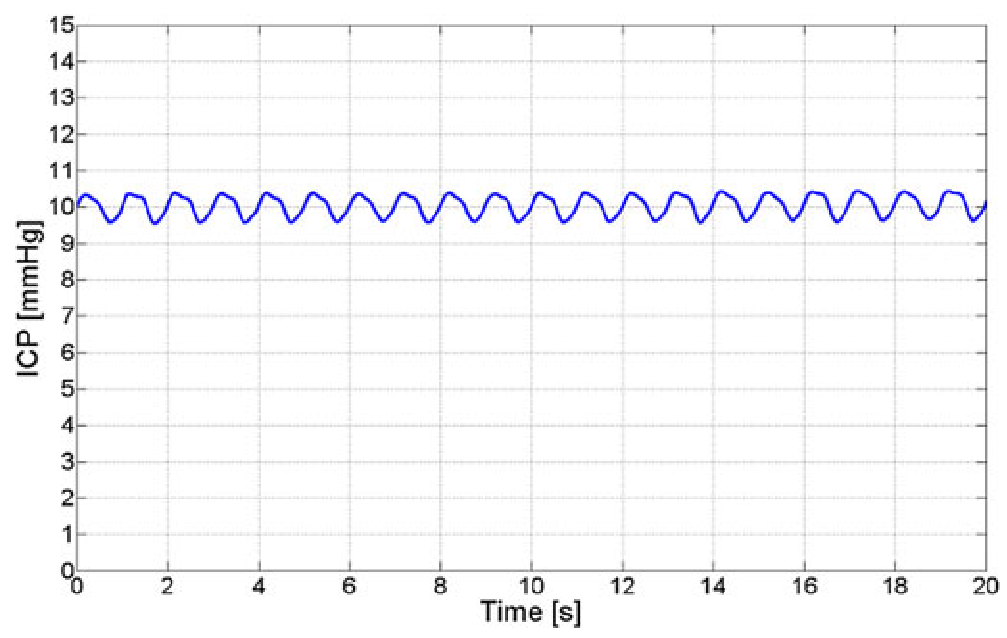
\includegraphics[width=0.7\textwidth]{Figures/5.png}
    \caption{在模拟体内测量的数个心动周期中的脑室内颅内压振荡。颅内压围绕10 mmHg的平均值以1 Hz的频率振荡。}
    \label{fig:results}
\end{figure}

\begin{figure}[h]
    \centering
    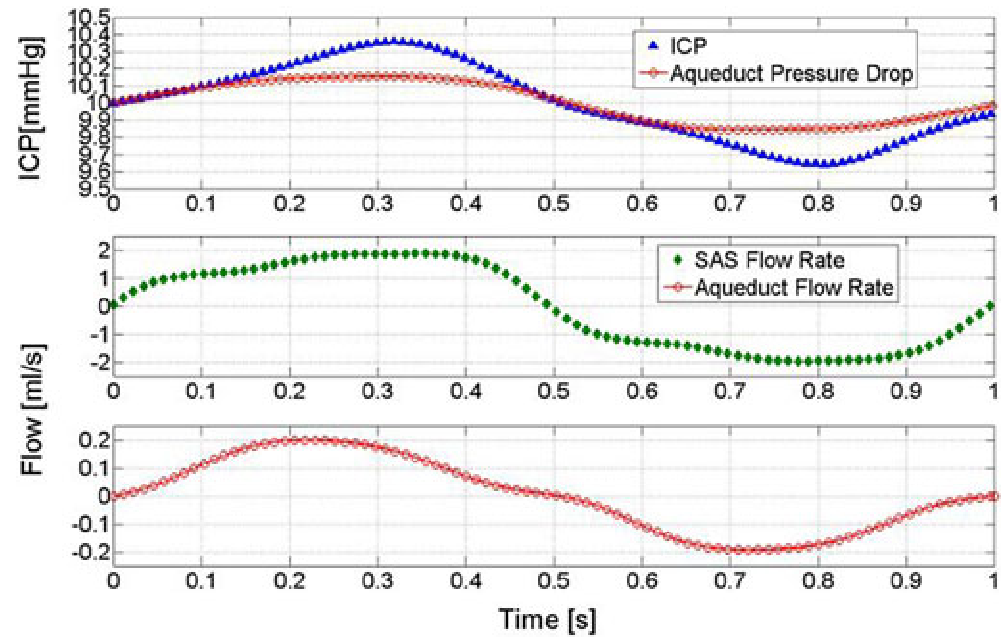
\includegraphics[width=0.7\textwidth]{Figures/6.png}
    \caption{在一个心脏周期内,模型中测量的颅内压(顶部)和脑脊液流速(底部)。(顶部)三角形标记显示了当脑脊液搏动起源于脑室和蛛网膜下腔时的颅内压;圆形标记表示仅在脑室搏动下的颅内压。(中间)导水管中的脑脊液流速。(底部)蛛网膜下腔中的脑脊液流速。}
    \label{fig:csf_flow}
\end{figure}
图\ref{fig:results}显示了模型在多个心脏周期中脑室内平均颅内压的记录,再现了 10 mmHg 的平均生理 ICP,并观察到幅度约为 0.4 mmHg 的脉动,展示了该装置的稳定性。
两者都与文献中报告的体内健康条件的数值一致。

一组典型心脏周期的瞬态ICP和相应的CSF流速曲线如图\ref{fig:csf_flow}所示。
CSF振荡在导水管中显示为0.2 ml/s的峰值,在SAS中则为2 ml/s的峰值,从而与体内值相匹配。
这是通过如II-E部分所述的脉动泵输出和精细调节阀设置的正确选择实现的。

为分析CSF脉动起源变化的影响,将整个脉动泵的输出施加到大脑表面,导致脑室脉动而没有SAS的贡献。
这使得ICP幅度从0.4 mmHg降低到0.15 mmHg,后者值对应于预期的导水管压力峰值下降。
当CSF脉动再次源自脑室和SAS中时,生理ICP幅度0.4 mmHg得以恢复。

\begin{figure}[!h]
    \centering
    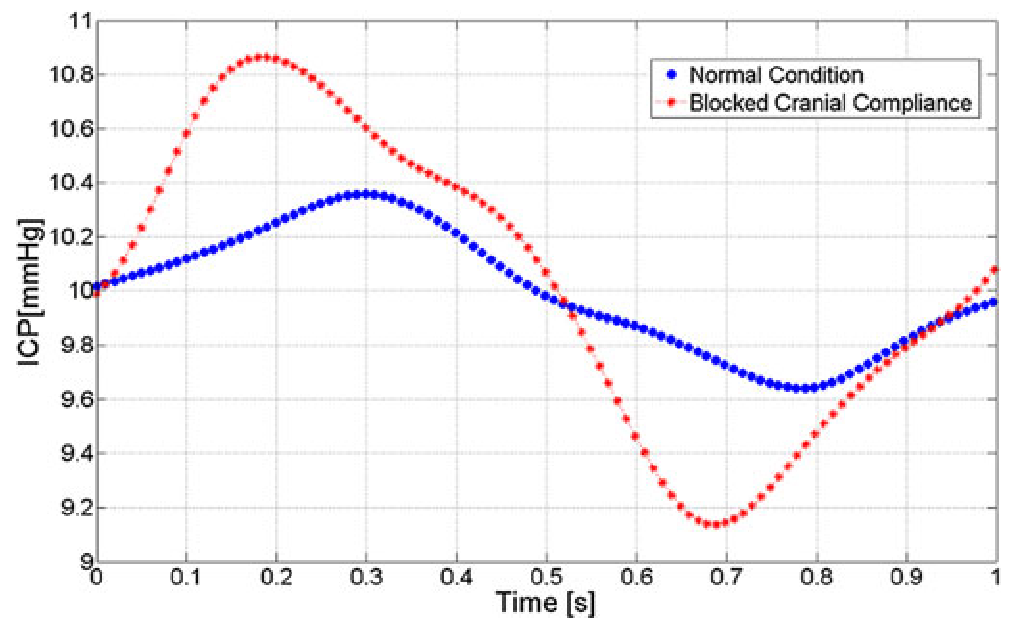
\includegraphics[width=0.6\textwidth]{Figures/7.png}
    \caption{在模型中进行的脑室内ICP脉动测量。比较正常顺应性下的健康状态(见表I)与无颅腔顺应性的病理状态。}
    \label{fig:icp_comparison}
\end{figure}

为了研究通过改变操作参数来使仿体灵活再现潜在病理状况的能力,我们将颅腔顺应性设置为零。
图\ref{fig:icp_comparison}显示了生理条件下的颅内压测量结果,比较了仿体中脑室内测得的颅内压脉动。健康状态具有正常顺应性(见表I)与无颅腔顺应性的病理状态进行了比较。在病理情况下观察到颅内压脉冲幅度增加了超过两倍。




\section*{\uppercase\expandafter{\romannumeral4}.讨论}

本文描述的模型代表了一种模拟颅内动力学的新方法。
基于MRI数据和详细的CFD模拟结果,实现了一个包括大脑、脑室和蛛网膜下腔的颅内空间模型,该模型允许重现监测体积和脉动的脑脊液流动以及颅内压动力学。
通过与文献中报道的生理脑脊液流动和压力值比较,对该模型进行了验证。

模型展示了一组操作参数,其生理值在体内无法轻易获得。
具体来说,这些参数是搏动泵的输出波形及其在脑室和蛛网膜下腔脑脊液空间的输出分配。
在体内,血管的扩张和收缩直接或间接通过瞬态脑组织运动推动脑脊液。由于这种复杂的相互作用迄今尚未完全量化,我们直接位移脑室壁和蛛网膜下腔体积的方法是合理的。
更重要的是,通过将搏动泵的输出和输出分配比作为变量,我们获得了指示,表明在体内脑脊液的振荡可能是蛛网膜下腔和心室体积的瞬态变化共同作用的结果,且幅度相似,而不是单一腔室体积变化的结果。
在模型中,相对贡献是以2:3偏向于蛛网膜下腔。

尽管在目前的状态下,模型尚未被验证用于病理状况的再现,我们仍然模拟了一种颅内顺应性降低的假设性疾病。
这是为了证明模型的操作参数可以轻松调整,以研究病理性颅内动力学。

正如所有模型一样,目前的模型是对非常复杂的真实系统的简化表示。特别是引入了简化来处理颅内空间的解剖复杂性。大脑血管及其对颅内动态的贡献隐含地体现在脑室和SAS腔室的体积变化中。
因此,血流的局部效应未得到考虑。同样,对脑室和SAS的简化阻碍了局部流动信息的获取。然而,模型仍在模拟的CSF空间内产生了逼真的压力动态。
在生理条件下,中脑水管和蛛网膜下腔(SAS)是脑脊液压力下降的主要原因,这两个室隔都在我们的设置中得到了准确的建模。
由于 Monro、Luschka 和 Magendie 孔的长度较短,侧脑室的横截面较大,它们的简化表示对整体压力动态和流速影响可以忽略不计。

虽然生理性颅内动态的带宽仅限于几个赫兹,但如同此处仅考虑其1赫兹的第一谐波无疑是一种明显的简化。
因此,测量的流动曲线形状并不完全匹配健康受试者所获得的那些,尽管振幅、平均流速和搏动量一致。
要详细再现体内流量曲线,需要一个带宽至少为10赫兹的更复杂的执行系统。
这将引入一大批需要校准的新变量,同时只提供非常有限的附加价值。

模型在空调房间中以22°C的温度操作,而不是在37°C的体温下。因此,工作流体(水)的密度和粘度比体内CSF [34] 的高。
这导致峰值压力梯度被高估约10\%。对于需要更准确反映CSF的应用,可以实施主动加热设置,或使用不同的工作流体。

颅脑模型中的恒定顺应性代表了健康状态下的有效假设。然而,在病理条件下,颅脊顺应性的变化可能变得重要。为研究这些情况,可以用文献[44]中报道的指数顺应性模块替换使用的恒定顺应性元件。

\end{document}
